% Gerado por scripts/gerar_secao_loa_pca_tcc.py a partir de resultados_loa_pca_2026/*.json. Não editar à mão.
\section{Aplicação ao planejamento orçamentário: LOA e PCA de 2026}
\label{sec:loa-pca-2026}
Esta seção aplica a previsão de demanda ao ciclo orçamentário. A pergunta é quanto o Estado deveria reservar na Lei Orçamentária Anual (LOA) de 2026 para a manutenção da frota, distribuído por órgão e por natureza de despesa, e que itens o Plano de Contratações Anual (PCA) de 2026 deveria prever, usando só dados observados até set/2025. O experimento está em scripts/planejamento\_loa\_pca\_2026.py; o confronto com a LOA e a execução, em scripts/execucao\_orcamentaria\_frota.py.
\subsection{Desenho e escolha do modelo}
A base de OS da SEA/SC tem cobertura completa até set/2025; depois disso restam poucas OS por mês, e esses meses foram tratados como ausentes. Os meses de out--dez/2025 foram presumidos pelo modelo. Três previsores (sazonal ingênuo com crescimento, ETS amortecido e SARIMA, os dois últimos em logaritmo) e a média deles foram avaliados em dois testes retrospectivos: treino até dez/2023 para prever 2024 e treino até dez/2024 para prever jan--set/2025. O critério foi o menor erro absoluto médio no total do período, e o escolhido foi o SARIMA (log), com 7,1\% (Tabela~\ref{tab:loa-backtest}).
\begin{table}[H]
\centering\small
\caption{Testes retrospectivos dos modelos de previsão do gasto anual de manutenção}
\label{tab:loa-backtest}
\begin{tabular}{p{0.08\textwidth}p{0.36\textwidth}p{0.15\textwidth}p{0.15\textwidth}p{0.13\textwidth}}
\hline
\textbf{Teste} & \textbf{Modelo} & \textbf{Previsto} & \textbf{Realizado} & \textbf{Erro no total} \\ \hline
BT1 & SNg (sazonal ingênuo com crescimento) & R\$ 30,86 mi & R\$ 32,36 mi & -4,7\% \\
BT1 & ETS amortecido (log) & R\$ 55,08 mi & R\$ 32,36 mi & 70,2\% \\
BT1 & SARIMA (log) & R\$ 30,97 mi & R\$ 32,36 mi & -4,3\% \\
BT1 & Média dos três & R\$ 38,97 mi & R\$ 32,36 mi & 20,4\% \\
BT2 & SNg (sazonal ingênuo com crescimento) & R\$ 25,10 mi & R\$ 21,94 mi & 14,4\% \\
BT2 & ETS amortecido (log) & R\$ 24,65 mi & R\$ 21,94 mi & 12,4\% \\
BT2 & SARIMA (log) & R\$ 24,10 mi & R\$ 21,94 mi & 9,8\% \\
BT2 & Média dos três & R\$ 24,62 mi & R\$ 21,94 mi & 12,2\% \\
\hline
\end{tabular}
\fonte{Elaborado pelo autor (2026).}
\end{table}
\begin{figure}[H]
\centering
\caption{Previsões mensais dos testes retrospectivos contra o realizado}
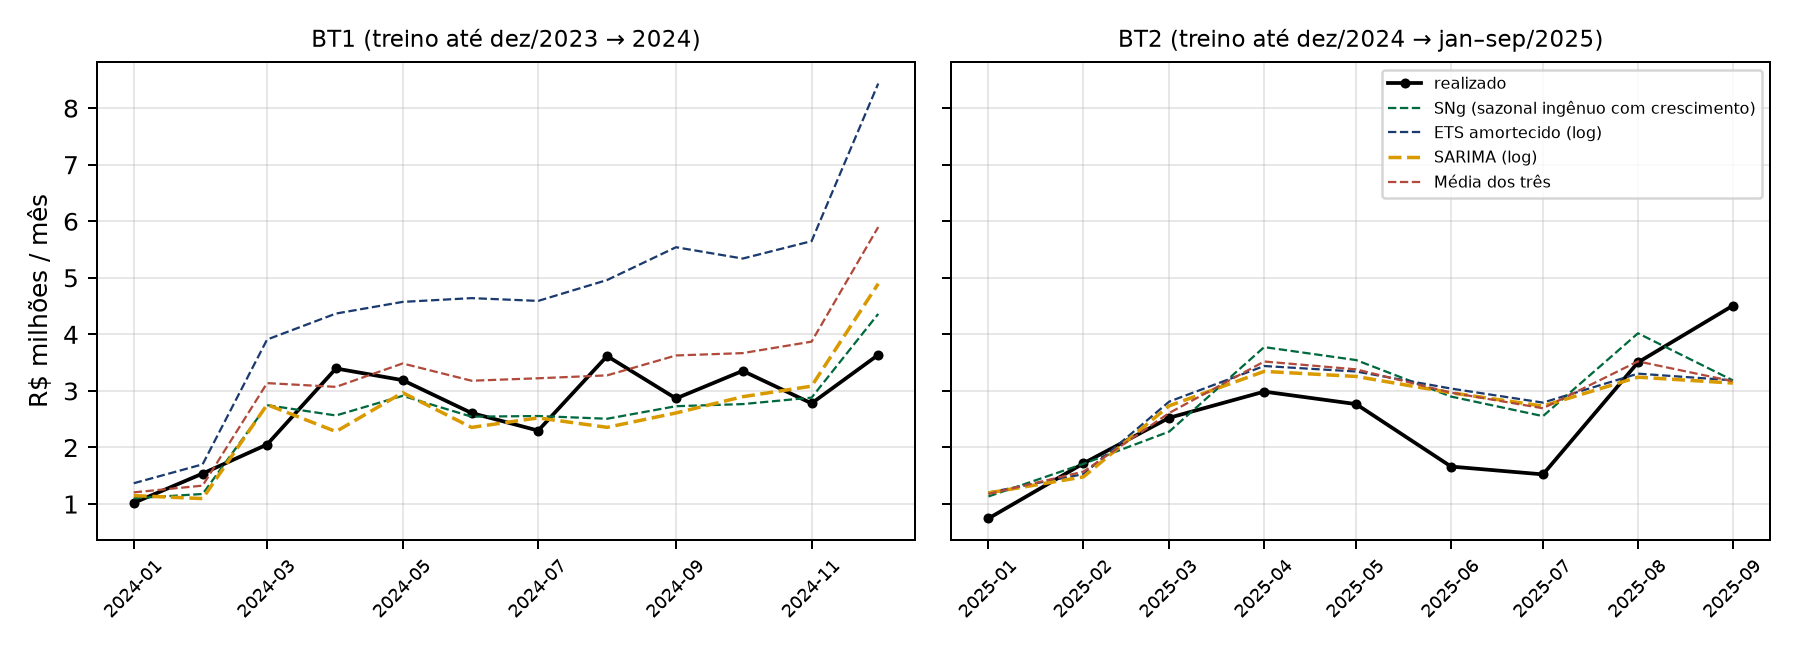
\includegraphics[width=0.95\textwidth]{figuras/loa2026_avaliacao_retrospectiva.png}
\fonte{Dados da SEA/SC e da SEF/SC processados pelo autor (2026).}
\label{fig:loa-backtest}
\end{figure}
\subsection{Proposta de LOA e de PCA}
A proposta para 2026 é de R\$ 33,59 mi, com intervalo de 80\% de R\$ 30,86 mi a R\$ 38,23 mi em 2.000 trajetórias simuladas do modelo. O valor fica 4,1\% acima de 2025 (observado e presumido, R\$ 32,28 mi) e 3,8\% acima de 2024 (R\$ 32,36 mi) (Figura~\ref{fig:loa-serie}). A distribuição por órgão usa a participação dos 12 meses até o corte; aplicadas ao total real de 2024, as participações de 2023 erraram 12,0\% do valor. Peças respondem por 67,5\% do gasto. O PCA proposto lista as 40 descrições de peça de maior gasto, que cobrem 57,6\% do valor de peças; 35 dos 40 maiores itens de 2024 já estavam entre os 40 maiores de 2023.
\begin{figure}[H]
\centering
\caption{Gasto mensal de manutenção: observado, meses presumidos e previsão de 2026}
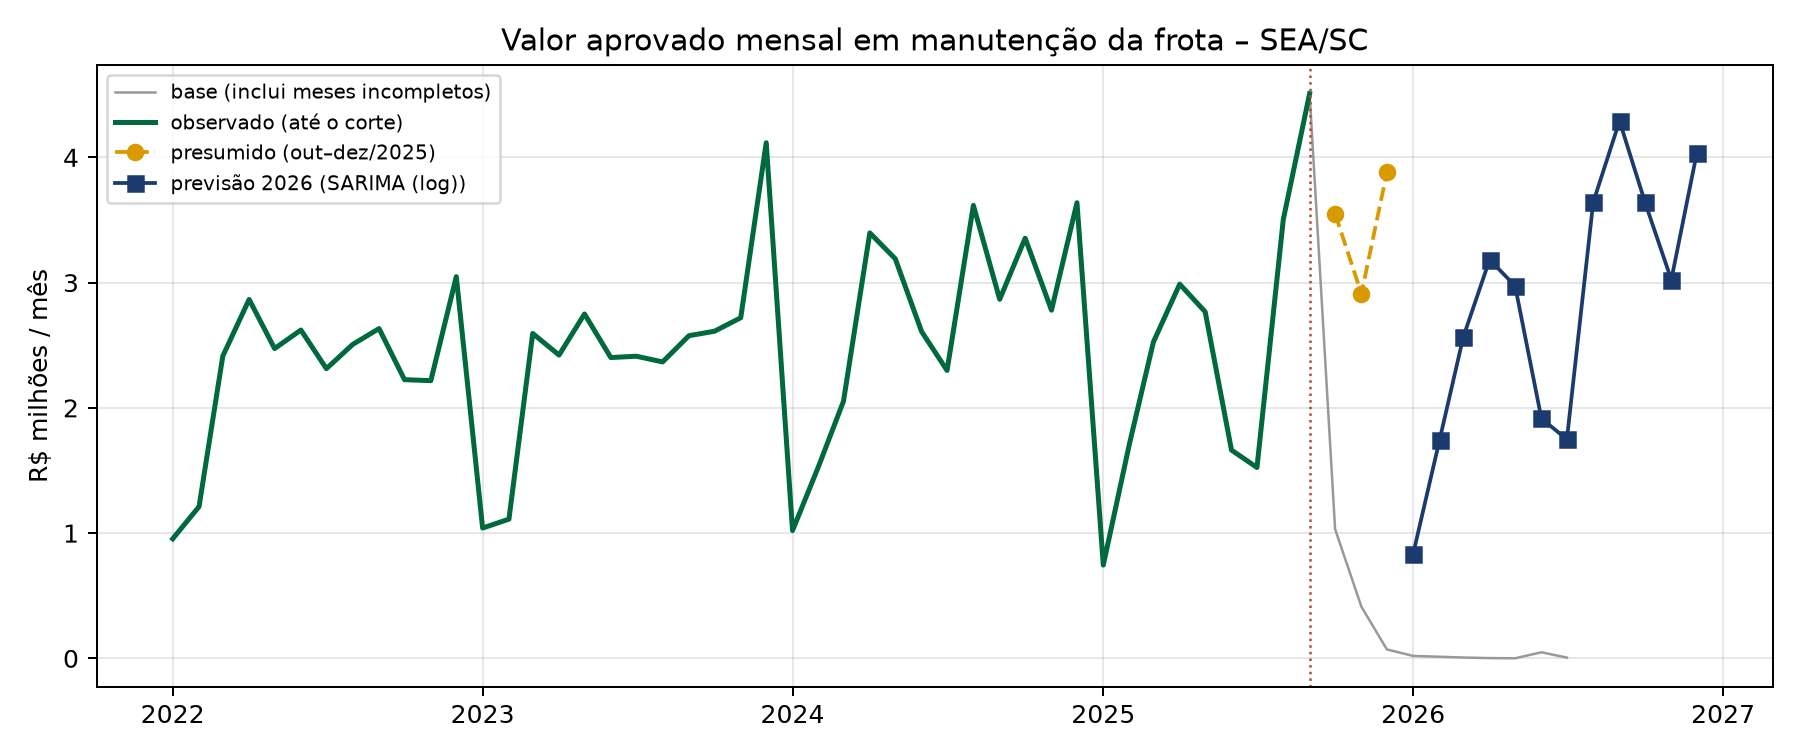
\includegraphics[width=0.95\textwidth]{figuras/loa2026_serie_previsao.png}
\fonte{Dados da SEA/SC e da SEF/SC processados pelo autor (2026).}
\label{fig:loa-serie}
\end{figure}
\begin{table}[H]
\centering\small
\caption{Proposta de LOA 2026 para manutenção da frota: seis maiores órgãos}
\label{tab:loa-orgaos}
\begin{tabular}{p{0.4\textwidth}p{0.14\textwidth}p{0.17\textwidth}p{0.17\textwidth}}
\hline
\textbf{Órgão} & \textbf{Participação} & \textbf{Proposta 2026} & \textbf{OS 2024} \\ \hline
PM SC & 51,5\% & R\$ 17,32 mi & R\$ 14,97 mi \\
SAP & 10,7\% & R\$ 3,60 mi & R\$ 4,71 mi \\
SES & 7,8\% & R\$ 2,64 mi & R\$ 3,11 mi \\
CBMSC & 5,3\% & R\$ 1,77 mi & R\$ 1,61 mi \\
PC SC & 4,9\% & R\$ 1,64 mi & R\$ 1,63 mi \\
SED & 3,8\% & R\$ 1,26 mi & R\$ 1,04 mi \\
\hline
\end{tabular}
\fonte{Elaborado pelo autor (2026).}
\end{table}
\subsection{Confronto com a LOA, o PCA e a execução de 2026}
A LOA 2026 (Lei nº 19.683/2026) foi lida por OCR. Ela identifica a frota em 2 subações de manutenção, 1 de combustível e 8 de aquisição; nos demais órgãos, inclusive a PM, a manutenção fica dentro de ações administrativas genéricas e não pode ser isolada.
\paragraph{Fonte da execução.} A execução foi medida nos empenhos da SEF/SC publicados em dados.sc.gov.br (conjunto ``empenhos'', 2024 a ago/2026), somando emissões e reforços e descontando anulações e estornos. Manutenção da frota corresponde aos subelementos 3.3.90.30.39 (material para manutenção de veículos) e 3.3.90.39.19 (manutenção e conservação de veículos), de todos os órgãos. Empenho é a reserva da despesa; ele não equivale ao valor liquidado nem ao aprovado nas OS.

\paragraph{Troca do contrato de manutenção.} Em 2024, Ticket Gestão em Manutenção EZC S.A. recebeu 96,2\% do empenho de manutenção. O primeiro empenho de QFrotas Sistemas Ltda. é de set/2025, e em 2026 essa empresa concentra 96,2\%. A base de OS da SEA/SC tem cobertura completa até set/2025, o mesmo mês da troca. A queda de OS depois do corte, tratada no experimento como fim da extração, coincide portanto com a mudança de contrato, o que indica que a base vem do sistema da contratada anterior. A projeção de 2026 estima um gasto que passou a correr em outro contrato, com outros preços e regras.

\paragraph{Escala das duas medidas.} Em 2024, único ano completo nas duas bases, o empenho de manutenção somou R\$ 37,65 mi e o valor aprovado nas OS da SEA/SC, R\$ 32,36 mi: o empenho foi 1,16 vez o valor das OS. Em 2025 o empenho foi R\$ 41,78 mi, contra R\$ 32,28 mi de OS observadas e presumidas.

\paragraph{Proposta do experimento contra o empenho de 2026.} De jan--ago/2026 foram empenhados R\$ 42,54 mi em manutenção, contra R\$ 30,78 mi e R\$ 31,93 mi no mesmo período de 2024 e 2025 (alta de 33,2\% sobre 2025). Esse valor já é 127\% da proposta anual do experimento (R\$ 33,59 mi) e 109\% da proposta convertida para a escala do empenho pela razão de 2024 (R\$ 39,08 mi). Parte da alta vem dos empenhos globais do novo contrato no início do ano: jan--mar/2026 concentram R\$ 32,08 mi. Se 2026 repetisse a fração empenhada até ago em 2024 (82\%) ou em 2025 (76\%), o ano fecharia entre R\$ 52,04 mi e R\$ 55,65 mi. Isso é uma indicação, não uma previsão, porque o novo contrato muda o calendário dos empenhos.

\paragraph{LOA: a subação da Polícia Civil.} A subação 702.0262.013148 (``Gestão da frota - PCSC'') tem R\$ 15,67 mi na LOA 2026, 9,5 vezes a proposta do experimento para a PC SC (R\$ 1,64 mi). Os empenhos explicam a diferença: em 2025 a subação empenhou R\$ 13,34 mi, dos quais R\$ 9,86 mi em combustível e só R\$ 1,84 mi em manutenção. Na mesma natureza de despesa, o empenho de manutenção de 2024 (R\$ 1,89 mi) fica perto das OS da SEA/SC (R\$ 1,63 mi) e da proposta. A distância vem do escopo da subação, que inclui combustível e locação, e não de erro da projeção.

\paragraph{LOA: demais subações da frota.} Fora da manutenção, a dotação inicial da LOA é um mau guia da execução: a subação de combustível da SIE e da PMRv tem R\$ 3,00 mi na LOA e já empenhou R\$ 3,45 mi (115\% da dotação inicial); a renovação da frota da SEJURI (R\$ 38,05 mi) não tinha empenho até ago/2026, depois de R\$ 18,30 mi em 2025; a aquisição de veículos do FES tem R\$ 5,15 mi na LOA, contra R\$ 25,38 mi empenhados em 2025; as subações de CELESC Distribuição S.A., CELESC Geração S.A., SC Participações e Parcerias S.A.(SCPAR) não têm empenho na base em nenhum dos três anos, o que é esperado para empresas estatais, cuja execução não passa pelo SIGEF; a subação 130.0089.014456 (``Modernização da frota de veículos, aeronaves e [\ldots{}]'', R\$ 2,50 mi) não teve empenho em 2024, 2025 nem até ago/2026. Na maior parte dos órgãos, inclusive a PM, a LOA não separa a frota, e a comparação só é possível pela natureza da despesa no empenho.

\paragraph{PCA 2026.} O PCA oficial não foi comparado: o PNCP respondeu com erro 503 ou tempo esgotado em todas as consultas.

\paragraph{Efeito sobre a hipótese exploratória E3.} A E3 (proposta com erro abaixo de 10\% no total) foi pré-registrada contra o valor aprovado nas OS de 2026 da SEA/SC, que ainda não foi extraído; o empenho é outra medida e não decide a hipótese. O sinal é desfavorável: mesmo na escala do empenho, o valor de jan--ago/2026 já supera a proposta anual em 9\% (a proposta para os mesmos meses é R\$ 18,61 mi), e a troca de contrato quebra a premissa de continuidade da série usada na projeção. Há também um risco para o próprio teste: se a extração de 2026 vier do sistema da contratada anterior, ela não terá as OS do novo contrato. Nesse caso a E3 não poderá ser testada como registrada, e qualquer troca de medida terá de ser registrada como desvio antes de ver os dados.

\begin{table}[H]
\centering\scriptsize
\caption{Manutenção da frota: empenho, OS da SEA/SC e proposta do experimento}
\label{tab:loa-execucao}
\begin{tabular}{p{0.30\textwidth}p{0.13\textwidth}p{0.15\textwidth}p{0.13\textwidth}p{0.17\textwidth}}
\hline
\textbf{Medida} & \textbf{2024} & \textbf{2025} & \textbf{2026 (jan--ago)} & \textbf{Proposta 2026} \\ \hline
Manutenção -- empenho (todos os órgãos) & R\$ 37,65 mi & R\$ 41,78 mi & R\$ 42,54 mi & R\$ 39,08 mi (esc. empenho) \\
Manutenção -- OS aprovadas SEA/SC & R\$ 32,36 mi & R\$ 32,28 mi (c/ presumido) & não extraído & R\$ 33,59 mi \\
PC SC subação 013148 -- total empenhado & R\$ 12,04 mi & R\$ 13,34 mi & R\$ 13,05 mi & LOA: R\$ 15,67 mi \\
PC SC subação 013148 -- só manutenção & R\$ 1,89 mi & R\$ 1,84 mi & R\$ 1,22 mi & R\$ 1,64 mi \\
PC SC -- OS aprovadas SEA/SC & R\$ 1,63 mi & — & — & — \\
\hline
\end{tabular}
\fonte{Empenhos SEF/SC (dados.sc.gov.br); OS da SEA/SC; elaborado pelo autor (2026).}
\end{table}
\begin{figure}[H]
\centering
\caption{Empenho acumulado de manutenção (2024--2026) contra a proposta do experimento, e subações da LOA 2026 que isolam a frota}
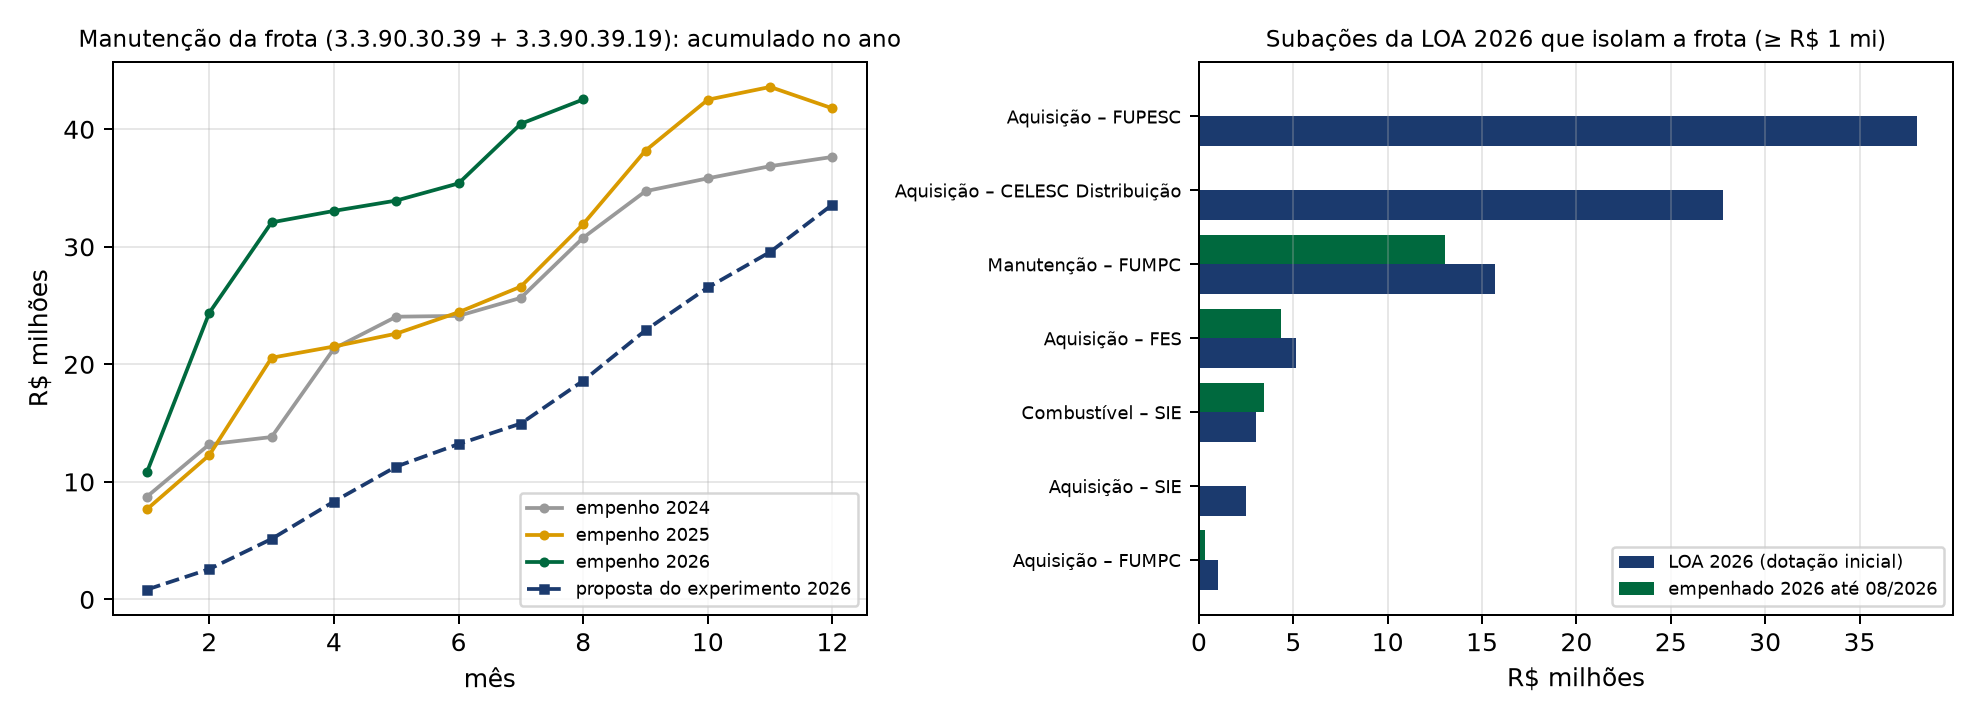
\includegraphics[width=0.95\textwidth]{figuras/loa2026_execucao_empenhos.png}
\fonte{Empenhos SEF/SC (dados.sc.gov.br), LOA 2026 e experimento; elaborado pelo autor (2026).}
\label{fig:loa-execucao}
\end{figure}
\subsection{Síntese}
\begin{itemize}
\item A proposta do experimento (R\$ 33,59 mi) subestima a execução de 2026: o empenho de jan--ago já a supera, também na escala do empenho.
\item Uma causa provável é a troca do contrato de manutenção em set/2025, que encerra a série da SEA/SC e muda preços e calendário.
\item As diferenças com a LOA vêm do escopo: a subação da PC SC inclui combustível e locação; na mesma natureza, empenho, OS e proposta ficam próximos.
\item A LOA só isola a frota em poucas subações; para os demais órgãos, a comparação precisa do empenho por subelemento.
\item O PCA oficial não pôde ser obtido (PNCP indisponível) e a E3 continua dependente da extração de 2026 da SEA/SC.
\end{itemize}
Para a gestão, o resultado tem duas leituras. O método reproduz bem um ano estável (erro médio de 7,1\% nos testes), mas não antecipa mudanças de contrato, que precisam entrar no planejamento como informação externa. E a LOA, no nível de subação, não serve para medir o custo da frota: o acompanhamento precisa usar a natureza da despesa nos empenhos, por subelemento, cruzada com as OS.
